This section introduces the concept of data mananagement layer, starting from its origin and evolution in to today's technologies. This dissertation includes advantages and limitations of each evolutive step, and describe the functions of \gls{DBMS}. what a data storage is and which typologies of storages exist. The subsections \ref{subsec:open_table_formats} explains in details the main \gls{DBMS} technologies of this project, namely Hudi, employed in the legacy version of Hopsworks feature store, Iceberg and Delta Lake, the two alternatives evaluated.

\subsection{Brief history of \glsfmtlongpl{DBMS}}
\label{subsec:history_DBMS}
Since the 2010s, with the advent of Big Data, the data volume, variety, and production velocity have increased exponentially \cite{ederUnstructuredData802008, penceWhatBigData2014}. While on one side, this proved to be of enormous value, on the other this posed several challenges \cite{demchenkoAddressingBigData2012} on data architectures, which had to evolve to cope with these new needs. Data lakehouse technologies, like Hudi, Iceberg and Delta Lake \cite{rajaperumalUberEngineeringIncremental2017,IcebergExamples2024,armbrustDeltaLakeHighperformance2020} are the last step of this evolution. However, to truly understand this tools, it is needed to start from the beginning of \gls{DBMS} evolution.

\smallskip

Before big data, companies already wanted to get insights from their data, automating the workflow from the data sources to point of access to this dataa. Here is where \gls{ETL} and relational databases first came into use. An \gls{ETL} pipeline consists of three steps:
\begin{enumerate}
    \item \textbf{Extracts} data from \glspl{API} or other various data sources.
    \item \textbf{Transforms} data according to one or more goal. Often this means removing absent fields, standardizes to a specific format to match the database schema, and validates the data.
    \item \textbf{Loads} it into a relational database (e.g., MySQL).
\end{enumerate}
This workflow structure enabled companies to generate \gls{BI} insights and data reports based on organizational data. However, a key limitation of this approach is its restricted ability to perform analytical queries that require joining multiple tables and working on several data dimensions. These types of queries, while executed less frequently than simpler queries, are essential for strategic decision-making (e.g., identifying the customer segment with the highest profitability over the past year, with the capabilities of drilling down on products, marketing and sales information).

\smallskip

To address the increasing demand for analytical queries, more advanced \glspl{DBMS} replaced traditional relational databases, optimizing performance for business-oriented analytical workloads. These systems, known as \glspl{OLAP}, introduced specialized storage and query execution strategies tailored for large-scale analytical processing. The most notable example of an \gls{OLAP} system is the data warehouse, which revolutionized how organizations handle structured data analysis. A data warehouse workflow, enables companies to process and analyze significantly larger datasets than traditional databases. Unlike transactional databases, which optimize for rapid insert/update operations, data warehouses focus on read-optimized queries by structuring data into columnar formats, reducing scan times for analytical queries. They maintain core relational database properties such as \gls{ACID} transactions and data versioning, ensuring data integrity and consistency for complex business intelligence applications.  

\smallskip

Over time, the exponential growth of unstructured data (e.g., images, videos, logs, and sensor data), posed new challenges for companies aiming to leverage such information. Traditional data warehouses struggled to accommodate this data due to their rigid schema requirements and high storage costs. Moreover, they were not designed to support \gls{AI}/\gls{ML} workflows that rely on diverse, unstructured datasets. To overcome these limitations, organizations adopted a new paradigm known as data lakes. Data lakes leverage cost-efficient object storage (Section~\ref{subsec:block_vs_file_vs_object}) and a schema-on-read approach, where raw data is loaded first and transformed only when needed. This shift from the traditional \gls{ETL} model to \gls{ELT} offers greater flexibility in handling diverse data types. For example, businesses can use data lakes to store raw IoT sensor readings and later refine them for predictive maintenance models, once the needed data transformation will be designed. 

\smallskip

Despite reducing storage costs and improving flexibility, data lakes introduced new complexities. Unlike structured databases, querying data lakes directly for \gls{BI} reports is impractical, as they lack indexing and transactional consistency. Additionally, maintaining separate storage solutions for structured (data warehouses) and unstructured (data lakes) data increases operational complexity and costs. A major drawback of data lakes is the risk of becoming "data swamps", repositories filled with ungoverned, low-quality data that provide little business value. Recognizing these challenges, organizations sought a hybrid solution combining the best features of data warehouses and data lakes. This led to the emergence of the data lakehouse architecture. First described by Databricks in 2020 at \gls{CIDR} \cite{lakehouse2021}, data lakehouses integrate structured and unstructured data storage while maintaining the governance, \gls{ACID} compliance, and indexing capabilities of data warehouses. The data lakehouse approach resolves many pain points associated with separate data warehouses and data lakes. It enables organizations to use the same storage for structured and unstructured data while supporting high-performance SQL queries and \gls{ML} workloads. By leveraging open columnar formats like Apache Parquet, ORC and Avro, data lakehouses ensure interoperability with various analytics engines. All these capabilities make lakehouses an ideal solution for enterprise-scale data processing. Table \ref{tab:DBMS_comparison} provides a comparison of data warehouses, data lakes, and data lakehouses, highlighting key takeaways for each technology.  

\begin{table}[h!]
    \centering
    \caption[Comparison of Data Technologies]{Comparison of Data Warehouses, Data Lakes, and Data Lakehouses \cite{inmonFiveStepsSuccessful}.}
    \label{tab:DBMS_comparison}
    \begin{tabular}{|p{2.3cm}|p{3.1cm}|p{3.1cm}|p{3.1cm}|}
        \hline
        \textit{\textbf{Feature}} & \textbf{Data Warehouse} & \textbf{Data Lake} & \textbf{Data Lakehouse} \\
        \hline
        \textit{Primary Use} & Business Intelligence, SQL Analytics & Unstructured data storage, AI/ML workflows & Unified storage for structured/unstructured data, SQL + AI/ML processing \\
        \hline
        \textit{Data Type} & Structured & Unstructured & All data types \\
        \hline
        \textit{Query Performance} & Optimized for SQL-based queries, fast indexed access & Slow for structured queries, requires extensive data preparation & High performance for both SQL and ML workloads \\
        \hline
        \textit{Schema Enforcement} & Strict schema-on-write & schema-on-read & Flexible schema with enforcement and evolution support \\
        \hline
        \textit{\gls{ACID} support} & Fully supported & Not supported & Fully supported \\
        \hline
        \textit{Scalability} & Limited scalability due to high storage costs & High scalability, low-cost storage & Highly scalable with structured query optimizations \\
        \hline
        \textit{Storage Cost} & High due to proprietary formats & Low due to object storage & Moderate, optimized for efficiency \\
        \hline
        \textit{Governance} & Strong governance, access control, and security & Weak governance, risk of data swamps & Fine-grained governance with access control and security \\
        \hline
        \textit{Key Takeaways} & Best for structured data and BI queries. High-performance SQL analytics. & Ideal for cost-effective big data storage. Difficult to manage and query efficiently & Combines the best of warehouses and lakes. Supports both SQL and AI/ML use cases efficiently. \\
        \hline
    \end{tabular}
\end{table}



\subsection{Open Table Formats}
\label{subsec:open_table_formats}

%%%%%% Modify this to include Apache Iceberg and Apache Hudi
The three main \gls{DBMS} technologies of this project are Hudi \cite{rajaperumalUberEngineeringIncremental2017}, Iceberg \cite{IcebergExamples2024} and Delta Lake \cite{armbrustDeltaLakeHighperformance2020}. These are also called \glspl{OTF} and they are the pivotal technology behind data lakehouses, serving as \glspl{DBMS} of those architectures. They provide an abstraction layer on top of data lakes, enabling database-like functionalities, enhancing data management capabilities significantly \cite{lakehouse2021,DataLakehouseSurvey2025}.

One of the cornerstone features of these formats is support for full \gls{CRUD} operations. This comprehensive functionality allows for flexible data manipulation and ensures that data lakes and warehouses can be updated in real time, reflecting the most current state of information. The ability to perform updates and deletes sets \glspl{OTF} apart from traditional file-based storage systems, where such operations are cumbersome and inefficient. Performance and scalability are other notable features that \glspl{OTF} bring to the table. These formats are designed to excel in Big Data environments, where data volumes are massive and continue to grow. They employ various optimization techniques, such as indexing, partitioning, and caching, to expedite data retrieval and processing. This not only improves query performance but also ensures that the system can scale horizontally to accommodate increasing data loads without a significant degradation in performance. As a result, organizations can manage their data ecosystems more effectively, making data-driven insights more accessible and actionable.Transactional support with \gls{ACID} compliance is another key feature of \glspl{OTF}. This ensures that all data transactions are processed reliably, maintaining data integrity and consistency across the board. This is particularly important in scenarios where multiple transactions occur simultaneously or when the system needs to recover from partial failures. \glspl{OTF} guarantee that each transaction is completed successfully or fully rolled back, providing an essential level of data reliability and trustworthiness for critical business operations. This feature is instrumental in supporting complex data workflows and ensuring that data lakes and warehouses can serve as a single source of truth for organizations.

Being \glspl{OTF} key components of the data lakehouse architecture, the increasing adoption of the data lakehouse architecture is reflected with the growth of the community of all three the technologies here discussed, as pictured in Figure \ref{fig:github_stars}


\begin{figure}[ht]
    \centering
    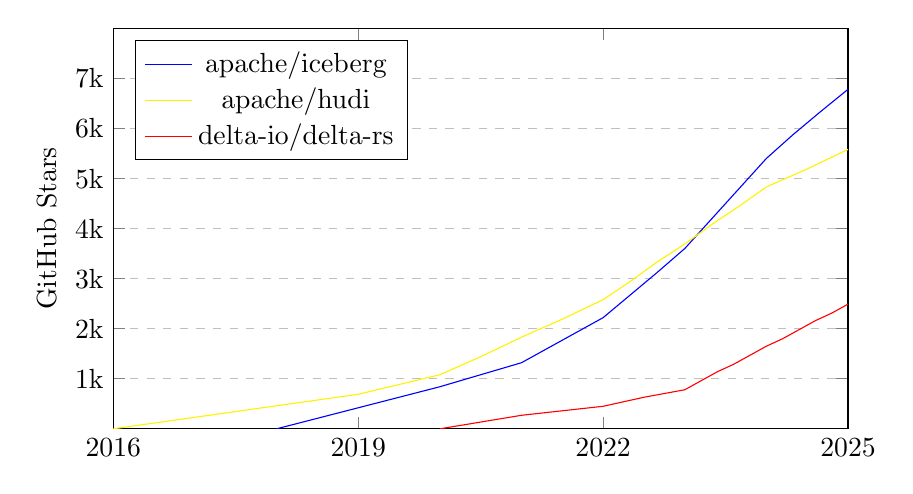
\begin{tikzpicture}
        \begin{axis}[
            ylabel={GitHub Stars},
            xmin=2016, xmax=2025,
            ymin=0, ymax=8000,
            xtick={2016, 2019, 2022, 2025},
            xticklabels={2016, 2019, 2022, 2025},
            ytick={1000, 2000, 3000, 4000, 5000, 6000, 7000},
            yticklabels={1k, 2k, 3k, 4k, 5k, 6k, 7k},
            legend pos=north west,
            ymajorgrids=true,
            grid style=dashed,
            width=0.9\textwidth, % Adjust width to fit the full space
            height=0.55\textwidth, % Adjust height for better proportions
        ] 
        \addplot[color=blue] coordinates {
            (2018, 0)
            (2020, 840)
            (2021, 1320)
            (2021.5, 1770)
            (2022, 2220)
            (2022.33, 2670)
            (2022.66, 3120)
            (2023, 3600)
            (2023.25, 4050)
            (2023.50, 4500)
            (2023.75, 4950)
            (2024, 5400)
            (2024.33, 5880)
            (2024.66, 6330)
            (2025, 6780)
        };
        \addlegendentry{apache/iceberg}
        \addplot[color=yellow] coordinates {
            (2016, 0)
            (2019, 690)
            (2020, 1080)
            (2020.5, 1440)
            (2021, 1830)
            (2021.5, 2190)
            (2022, 2580)
            (2022.33, 2940)
            (2022.66, 3330)
            (2023, 3690)
            (2023.33, 4080)
            (2023.66, 4440)
            (2024, 4830)
            (2024.5, 5190)
            (2025, 5580)
        };
        \addlegendentry{apache/hudi}
        \addplot[color=red] coordinates {
            (2020, 0)
            (2021, 270)
            (2022, 450)
            (2022.5, 630)
            (2023, 780)
            (2023.2, 960)
            (2023.4, 1140)
            (2023.6, 1290)
            (2023.8, 1470)
            (2024, 1650)
            (2024.2, 1800)
            (2024.4, 1980)
            (2024.6, 2160)
            (2024.8, 2310)
            (2025, 2490)
        };
        \addlegendentry{delta-io/delta-rs}
        \end{axis}
    \end{tikzpicture}
    \caption[GitHub stars of \glspl{OTF} repositories]{Trend of GitHub stars for \href{https://github.com/apache/iceberg}{apache/iceberg}, \href{https://github.com/apache/hudi}{apache/hudi}, and \href{https://github.com/delta-io/delta-rs}{delta-io/delta-rs} repositories.}
    \label{fig:github_stars}
\end{figure}



Delta Lake is the technology that will be most used in this project. A Delta Lake Table (i.e., an instance of Delta Lake) operates on a data lake containing Parquet files and a transaction log. The transaction log records each operation, enabling versioning and recovery of previous versions (also called time travel). The data lake can be partitioned, e.g., using a date field, making the Delta Lake table look like Figure \ref{fig:delta_table}


\subsubsection*{Apache Hudi}
\subsubsection*{Apache Iceberg}
\subsubsection*{Delta Lake}